%!TEX root = ../template.tex
%%%%%%%%%%%%%%%%%%%%%%%%%%%%%%%%%%%%%%%%%%%%%%%%%%%%%%%%%%%%%%%%%%%
%% chapter1.tex
%% NOVA thesis document file
%%
%% Chapter with introduction
%%%%%%%%%%%%%%%%%%%%%%%%%%%%%%%%%%%%%%%%%%%%%%%%%%%%%%%%%%%%%%%%%%%
\typeout{NT FILE chapter4.tex}%

\chapter{Advanced Feedback}
\label{chap:algo}

Providing meaningful feedback is a complex challenge. In this section, we present the key elements that would contribute to producing meaningful feedback, along with a potential solution using an algorithm that is currently under development. This concept is still in the research phase, and some aspects remain unsolved. However, initial scripts have been developed to explore its feasibility and support some of the claims made in this text. 

\section{Feedback Components}
To develop an advanced feedback system for \gls{ND} exercises, we first need to define its key components. An effective system should provide relevant information to assist students in solving proofs, making the process more teaching-like. With this in mind, we identify three fundamental aspects of a well-designed feedback system:

\begin{itemize}
    \item \textbf{Providing guidance on rule applications:} Some rule applications in \gls{ND} are not obvious, making it difficult for students to progress. The system should identify such situations and suggest applicable rules. When students are unsure how to proceed, it can also provide step-by-step guidance or even a complete resolution, depending on the proficiency level.
    
    \item \textbf{Breaking proofs into smaller sub-proofs:} To simplify reasoning, the feedback should allow students to focus on smaller proofs. By dividing proofs into smaller steps, it will reduce the cognitive load and encourage incremental learning.
    
    \item \textbf{Indicating the distance to a solution:} Showing how many steps (rule applications) are needed to complete the proof helps students maintain focus and gain a clear sense of progress.
\end{itemize}

These components offer several advantages in the learning process. By providing structured and clear information, the system becomes more robust, helping students overcome challenges throughout the proof.

In the next section, we present an algorithm that is still under development and addresses the previously mentioned points.

\section{Algorithm}
Research has already started on developing an algorithm to provide the previously mentioned components. The motivation behind this algorithm is the lack of development tools that offer meaningful and powerful feedback for \gls{ND}. While some tools were referenced in Section \ref{chap:assistants}, they do not fully address the feedback components. By designing our own algorithm with a focus on these components, we gain greater control over the assistance system, ensuring a more adaptable and effective environment.

The complexity of \gls{ND} proofs, with their multiple rules (as outlined in \ref{sec:pl_rules} and \ref{sec:fol_rules}), presents a challenge. Some rules generate multiple branches, while others introduce new elements into the proof. Developing an algorithm to handle this complexity is not a simple task. The algorithm we present is based on the Bounded Model Checking (BMC) algorithm~\cite{biere2021bounded}, but with a different purpose. BMC is traditionally used in verification, where it checks whether a system violates a given property by searching for counterexamples within a finite execution trace. It encodes the system and property into a SAT\footnote{SAT (Satisfiability Problem) is a well-known problem in logic, where the goal is to determine if there exists a valuation that makes a given boolean expression satisfiable~\cite{You2019G2SATLT}. SAT formulas are logical expressions typically written in Conjunctive Normal Form (CNF), which is a conjunction of disjunctions.} formula and verifies correctness within a bounded number of steps. In contrast, our version of the algorithm shifts the focus from verification to structured solution generation. Instead of identifying counterexamples, we use the algorithm to generate a bounded graph of states that will store solutions within a certain range.

In the graph, each node represents a distinct state within the proof. By state, we refer to the logical expressions in the \gls{ND} proof, which, at different stages, can have available different sets of hypotheses. Below is an example where, in step \textbf{A} (at the beginning of the proof), the expression \(a \to (a \lor b)\) has no hypotheses available. In contrast, in step \textbf{B} (later in the proof), the same expression has \(\neg(a \to (a \lor b))\) as a hypothesis.

\[
\begin{array}{c c}
   \quad \frac{\displaystyle \frac{\displaystyle 
    {\displaystyle \textbf{B.} \quad a \to (a \lor b) \strut} \quad \quad \neg(a \to (a \lor b))^1 \quad \strut} {\displaystyle \bot \strut} \quad (\neg E) \strut}
    {\displaystyle \textbf{A.} \quad a \to (a \lor b)\strut} \quad (\bot, 1) 
\end{array}
\]

Each edge represents the application of a rule, transitioning from one state to another. Some edges have constraint expressions, which means the algorithm can only move to the next stage if the current state contains the corresponding constraint in its set of hypotheses (represented in red). Other edges can generate new hypotheses that are added to the set of hypotheses (represented in blue). Figure \ref{img:algorithm} illustrates an example of a graph that can be used to prove \(a \to (a \lor b)\).

\begin{figure}[htbp]
    \centering
    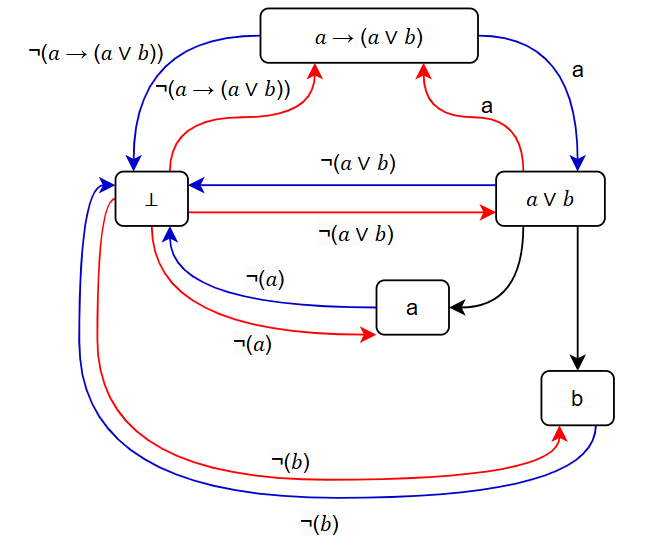
\includegraphics[width=0.5\linewidth]{algorithm}
    \caption{Graph to prove \(a \to (a \lor b)\).}
    \label{img:algorithm}
\end{figure}

There are potential questions that may arise. The first one might be: How do we build the graph? To build the graph, we first need to compute the different states. For that, we will need to apply rules successively to the expression we want to prove, generating hypotheses at each step. Then, starting with the hypotheses previously generated and using the provided premises, we will attempt to decompose them further by applying the rules again and breaking them down into smaller components until we find a point of connection between the derived expressions. As we proceed with this process, we can begin constructing the state machine, using the rules applied to generate the new states.

This could lead to the question, "How will we extract a solution from the graph?" To find a solution, we need to traverse the entire graph by testing all combinations of paths starting from the conclusion and verifying if, using the list of hypotheses in each state, we can close the current node. This can be a computationally intensive operation since we have loops and may pass through the same operations multiple times. To address this, we will define a depth limit for the proofs, selecting an appropriate value based on the typical size of proofs. Increasing this limit unnecessarily would lead to an exponential growth in the number of possible combinations. There are also ways to avoid looping through unnecessary paths, which can significantly increase the efficiency of the algorithm. A possible solution for \(a \to (a \lor b)\) using the graph in \ref{img:algorithm} would be \(\boxed{a \to (a \lor b)} \Rightarrow \boxed{\vphantom{a \to (a \lor b)}a \lor b} \Rightarrow \boxed{\vphantom{a \to (a \lor b)}a}\), since we can close \(a\) using the hypothesis that we collect from transitioning from \(\boxed{a \to (a \lor b)} \Rightarrow \boxed{\vphantom{a \to (a \lor b)}a \lor b}\).

Another question that may come up is, "How will this algorithm adapt to the user's solution?". To handle that, we first need to check if the set of the student's derived expressions aligns with those generated by the algorithm. If there is a mismatch, we will expand the graph by adding the new expressions and derivations from those expressions, in the same way the graph was initially constructed. Once the graph is updated, we can select one of the open leaves in the student's proof and query the algorithm by providing the leaf and its state in the student's solution.

However, there are certain challenges that we have not yet fully addressed, such as how to handle rules that generate multiple branches, like the Disjunction Elimination rule. Despite these challenges, we believe this is a solid starting point for developing an effective algorithm. The algorithm is sound, meaning it will only generate valid proofs, but it is not complete due to the imposed restrictions on proof size and the set of derived expressions.

If we can efficiently implement this algorithm and incorporate rules that generate multiple branches, we will be able to create a highly effective feedback and hint system. This algorithm will address all the key components previously mentioned. Since it can adapt to the user's solution and find solutions, it can be used to provide guidance on rule applications, assist in breaking down the proof into sub-goals, and indicate the distance to a solution, as the algorithm is aware of the steps required to complete the proof.

As mentioned earlier, this is still a concept under study, and some of the topics discussed remain somewhat abstract.

\subsection{Results}
In this section, we present some results of the key features of our current algorithm. We will use the proof \((P \to (Q \to R)) \to (P \to Q) \to (P \to R)\) as an example to illustrate these features.

\begin{itemize}
    \item \textbf{Query full proofs:} The algorithm can be used to find multiple possible solutions to a given problem. For example, Figure \ref{img:algo2} shows the output from running the algorithm, and Figure \ref{img:algo1} displays the corresponding deduction tree. In the output, each line represents a formula from the tree, with the TAB indentation indicating the tree's structure. In our current implementation, we are not keeping track of the rule names, but in the output we can still deduce which rule was applied by examining the hypotheses at each expression and the number of children. The algorithm uses Breadth-First Search (BFS)\footnote{Breadth-First Search (BFS) is an algorithm used to traverse or search through graphs and trees. It explores the nodes level by level, starting from the root or source node, visiting all nodes at the current depth before moving on to the next level.} to find potential solutions. The characteristics of BFS ensure that the output always returns the shortest solution to the problem.

    \begin{figure}[htbp]
        \centering
        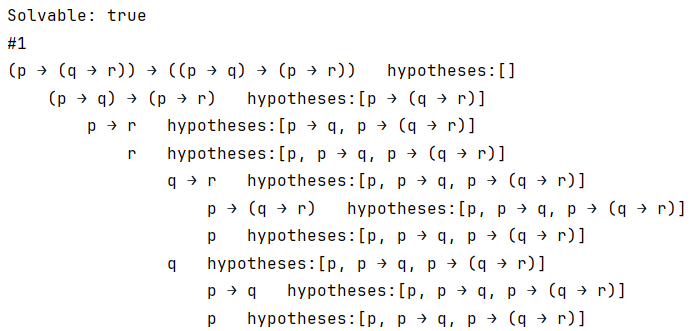
\includegraphics[width=0.9\linewidth]{algo2}
        \caption{Algorithm proving \((P \to (Q \to R)) \to (P \to Q) \to (P \to R)\).}
        \label{img:algo2}
    \end{figure}

    \begin{figure}[htbp]
        \centering
        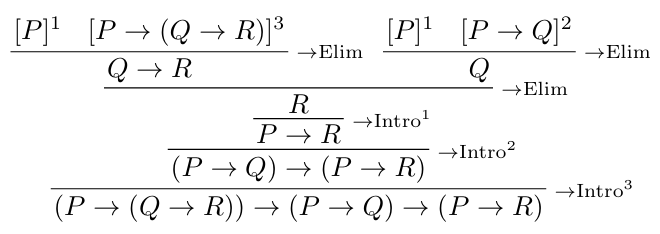
\includegraphics[width=0.7\linewidth]{algo1}
        \caption{Deduction tree for \((P \to (Q \to R)) \to (P \to Q) \to (P \to R)\).}
        \label{img:algo1}
    \end{figure}
        
    \item \textbf{Query parts of the proof:} The algorithm can also be used to query specific parts of the proof by providing the state we wish to complete. For instance, in Figure \ref{img:algo3} we want to finish the proof, but we do not know how to proceed. By querying the algorithm with our current state in this case the expression \(R\) with the hypotheses \(\{P \to (Q \to R), P \to Q, P\}\) the algorithm can find solutions for that state. Figure \ref{img:algo4} shows the result of this query.

    \begin{figure}[htbp]
        \centering
        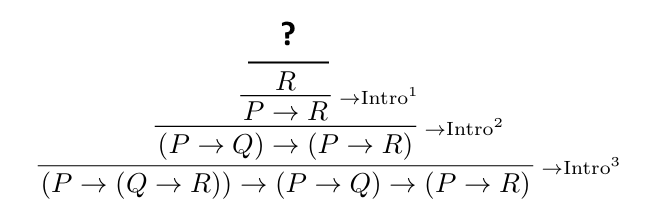
\includegraphics[width=0.7\linewidth]{algo3}
        \caption{Incomplete proof.}
        \label{img:algo3}
    \end{figure}
        
    \begin{figure}[htbp]
        \centering
        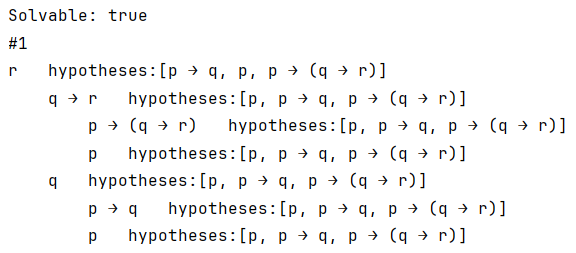
\includegraphics[width=0.8\linewidth]{algo4}
        \caption{Result of querying the algorithm using expression \(R\) and hypotheses \(\{P \to (Q \to R), P \to Q, P\}\).}
        \label{img:algo4}
    \end{figure}
\end{itemize}




